% Options for packages loaded elsewhere
\PassOptionsToPackage{unicode}{hyperref}
\PassOptionsToPackage{hyphens}{url}
%
\documentclass[
  ignorenonframetext,
]{beamer}
\usepackage{pgfpages}
\setbeamertemplate{caption}[numbered]
\setbeamertemplate{caption label separator}{: }
\setbeamercolor{caption name}{fg=normal text.fg}
\beamertemplatenavigationsymbolsempty
% Prevent slide breaks in the middle of a paragraph
\widowpenalties 1 10000
\raggedbottom
\setbeamertemplate{part page}{
  \centering
  \begin{beamercolorbox}[sep=16pt,center]{part title}
    \usebeamerfont{part title}\insertpart\par
  \end{beamercolorbox}
}
\setbeamertemplate{section page}{
  \centering
  \begin{beamercolorbox}[sep=12pt,center]{part title}
    \usebeamerfont{section title}\insertsection\par
  \end{beamercolorbox}
}
\setbeamertemplate{subsection page}{
  \centering
  \begin{beamercolorbox}[sep=8pt,center]{part title}
    \usebeamerfont{subsection title}\insertsubsection\par
  \end{beamercolorbox}
}
\AtBeginPart{
  \frame{\partpage}
}
\AtBeginSection{
  \ifbibliography
  \else
    \frame{\sectionpage}
  \fi
}
\AtBeginSubsection{
  \frame{\subsectionpage}
}
\usepackage{amsmath,amssymb}
\usepackage{lmodern}
\usepackage{iftex}
\ifPDFTeX
  \usepackage[T1]{fontenc}
  \usepackage[utf8]{inputenc}
  \usepackage{textcomp} % provide euro and other symbols
\else % if luatex or xetex
  \usepackage{unicode-math}
  \defaultfontfeatures{Scale=MatchLowercase}
  \defaultfontfeatures[\rmfamily]{Ligatures=TeX,Scale=1}
\fi
% Use upquote if available, for straight quotes in verbatim environments
\IfFileExists{upquote.sty}{\usepackage{upquote}}{}
\IfFileExists{microtype.sty}{% use microtype if available
  \usepackage[]{microtype}
  \UseMicrotypeSet[protrusion]{basicmath} % disable protrusion for tt fonts
}{}
\makeatletter
\@ifundefined{KOMAClassName}{% if non-KOMA class
  \IfFileExists{parskip.sty}{%
    \usepackage{parskip}
  }{% else
    \setlength{\parindent}{0pt}
    \setlength{\parskip}{6pt plus 2pt minus 1pt}}
}{% if KOMA class
  \KOMAoptions{parskip=half}}
\makeatother
\usepackage{xcolor}
\newif\ifbibliography
\usepackage{color}
\usepackage{fancyvrb}
\newcommand{\VerbBar}{|}
\newcommand{\VERB}{\Verb[commandchars=\\\{\}]}
\DefineVerbatimEnvironment{Highlighting}{Verbatim}{commandchars=\\\{\}}
% Add ',fontsize=\small' for more characters per line
\usepackage{framed}
\definecolor{shadecolor}{RGB}{248,248,248}
\newenvironment{Shaded}{\begin{snugshade}}{\end{snugshade}}
\newcommand{\AlertTok}[1]{\textcolor[rgb]{0.94,0.16,0.16}{#1}}
\newcommand{\AnnotationTok}[1]{\textcolor[rgb]{0.56,0.35,0.01}{\textbf{\textit{#1}}}}
\newcommand{\AttributeTok}[1]{\textcolor[rgb]{0.77,0.63,0.00}{#1}}
\newcommand{\BaseNTok}[1]{\textcolor[rgb]{0.00,0.00,0.81}{#1}}
\newcommand{\BuiltInTok}[1]{#1}
\newcommand{\CharTok}[1]{\textcolor[rgb]{0.31,0.60,0.02}{#1}}
\newcommand{\CommentTok}[1]{\textcolor[rgb]{0.56,0.35,0.01}{\textit{#1}}}
\newcommand{\CommentVarTok}[1]{\textcolor[rgb]{0.56,0.35,0.01}{\textbf{\textit{#1}}}}
\newcommand{\ConstantTok}[1]{\textcolor[rgb]{0.00,0.00,0.00}{#1}}
\newcommand{\ControlFlowTok}[1]{\textcolor[rgb]{0.13,0.29,0.53}{\textbf{#1}}}
\newcommand{\DataTypeTok}[1]{\textcolor[rgb]{0.13,0.29,0.53}{#1}}
\newcommand{\DecValTok}[1]{\textcolor[rgb]{0.00,0.00,0.81}{#1}}
\newcommand{\DocumentationTok}[1]{\textcolor[rgb]{0.56,0.35,0.01}{\textbf{\textit{#1}}}}
\newcommand{\ErrorTok}[1]{\textcolor[rgb]{0.64,0.00,0.00}{\textbf{#1}}}
\newcommand{\ExtensionTok}[1]{#1}
\newcommand{\FloatTok}[1]{\textcolor[rgb]{0.00,0.00,0.81}{#1}}
\newcommand{\FunctionTok}[1]{\textcolor[rgb]{0.00,0.00,0.00}{#1}}
\newcommand{\ImportTok}[1]{#1}
\newcommand{\InformationTok}[1]{\textcolor[rgb]{0.56,0.35,0.01}{\textbf{\textit{#1}}}}
\newcommand{\KeywordTok}[1]{\textcolor[rgb]{0.13,0.29,0.53}{\textbf{#1}}}
\newcommand{\NormalTok}[1]{#1}
\newcommand{\OperatorTok}[1]{\textcolor[rgb]{0.81,0.36,0.00}{\textbf{#1}}}
\newcommand{\OtherTok}[1]{\textcolor[rgb]{0.56,0.35,0.01}{#1}}
\newcommand{\PreprocessorTok}[1]{\textcolor[rgb]{0.56,0.35,0.01}{\textit{#1}}}
\newcommand{\RegionMarkerTok}[1]{#1}
\newcommand{\SpecialCharTok}[1]{\textcolor[rgb]{0.00,0.00,0.00}{#1}}
\newcommand{\SpecialStringTok}[1]{\textcolor[rgb]{0.31,0.60,0.02}{#1}}
\newcommand{\StringTok}[1]{\textcolor[rgb]{0.31,0.60,0.02}{#1}}
\newcommand{\VariableTok}[1]{\textcolor[rgb]{0.00,0.00,0.00}{#1}}
\newcommand{\VerbatimStringTok}[1]{\textcolor[rgb]{0.31,0.60,0.02}{#1}}
\newcommand{\WarningTok}[1]{\textcolor[rgb]{0.56,0.35,0.01}{\textbf{\textit{#1}}}}
\setlength{\emergencystretch}{3em} % prevent overfull lines
\providecommand{\tightlist}{%
  \setlength{\itemsep}{0pt}\setlength{\parskip}{0pt}}
\setcounter{secnumdepth}{-\maxdimen} % remove section numbering
\ifLuaTeX
  \usepackage{selnolig}  % disable illegal ligatures
\fi
\IfFileExists{bookmark.sty}{\usepackage{bookmark}}{\usepackage{hyperref}}
\IfFileExists{xurl.sty}{\usepackage{xurl}}{} % add URL line breaks if available
\urlstyle{same} % disable monospaced font for URLs
\hypersetup{
  pdftitle={pfR},
  hidelinks,
  pdfcreator={LaTeX via pandoc}}

\title{\texttt{pfR}}
\author{Taylor R. Brown\\
Dept. of Statistics\\
University of Virginia}
\date{2023-06-23}

\begin{document}
\frame{\titlepage}

\begin{frame}{State-space models!}
\protect\hypertarget{state-space-models}{}
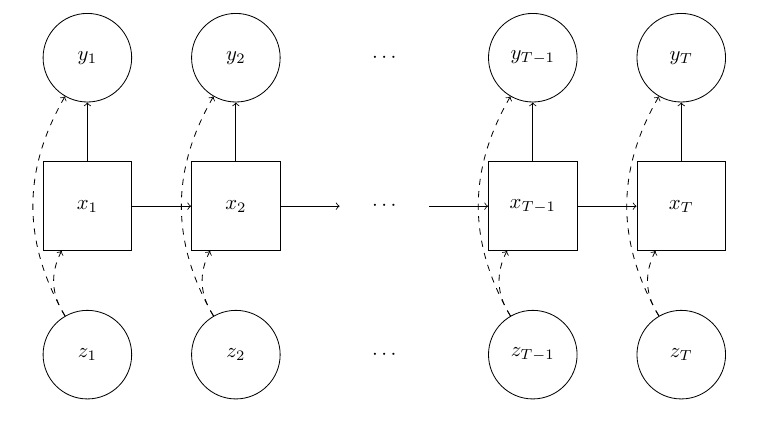
\includegraphics[width=1\linewidth]{pics/ssm_diagram_1-1}

\(\{y_t\}\): time series, \(\{x_t\}\): hidden states, \(\{z_t\}\):
inputs
\end{frame}

\begin{frame}{State-space models}
\protect\hypertarget{state-space-models-1}{}
Defining a state-space model requires defining

\begin{itemize}
\tightlist
\item
  \(g(y_t \mid x_t, \theta)\) observation distributions,
\item
  \(f(x_t \mid x_{t-1}, \theta)\) state transition distributions, and
\item
  \(\mu(x_t \mid \theta)\) an initial state distribution.
\end{itemize}

If you're Bayesian, you might also pick a prior \(\pi(\theta)\).
\end{frame}

\begin{frame}{Inference}
\protect\hypertarget{inference}{}
Statistical inference can target:

\begin{itemize}
\tightlist
\item
  states (assuming parameters are known),
\item
  parameters (ignoring states), or
\item
  both states and parameters simultaneously.
\end{itemize}
\end{frame}

\begin{frame}{State Inference}
\protect\hypertarget{state-inference}{}
Filtering distributions are

\begin{itemize}
\tightlist
\item
  \(p(x_t \mid y_{1:t}, \theta)\),
\item
  found by recursively applying Bayes' rule,
\item
  a tool for forecasting, and
\item
  approximated with \textbf{weighted samples} in particle filters.
\end{itemize}
\end{frame}

\begin{frame}{Parameter Inference}
\protect\hypertarget{parameter-inference}{}
The likelihood \(p(y_{1:T} \mid \theta)\) is the difficult part!

\begin{itemize}
\tightlist
\item
  Frequentists have difficulty optimizing it.
\item
  Bayesians have difficulty integrating it.
\end{itemize}

Particle filters give us a \textbf{random approximate evaluation} of it.
\end{frame}

\begin{frame}{Problems}
\protect\hypertarget{problems}{}
Unfortunately, particle filters are tricky business:

\begin{itemize}
\tightlist
\item
  running them in interpreted languages is slow,
\item
  writing them in compiled code is slow,
\item
  there are so many to choose from, and
\item
  they're difficult or impossible to parallelize.
\end{itemize}
\end{frame}

\begin{frame}[fragile]{The Solution}
\protect\hypertarget{the-solution}{}
\texttt{pfR} is the R interface to \texttt{pf} (a C++ particle filtering
library).

\texttt{pf} is fast, but\ldots{}

\begin{itemize}
\tightlist
\item
  lots of boilerplate
\item
  pure C++
\end{itemize}
\end{frame}

\begin{frame}[fragile]{The Solution}
\protect\hypertarget{the-solution-1}{}
\texttt{pfR} automatically generates 99\% of the code!

Each model/algorithm pair gets its own class. For each pair, generate

\begin{enumerate}
\tightlist
\item
  a header file,
\item
  source file with model definition, and
\item
  export code to use c++ stuff from within R.
\end{enumerate}
\end{frame}

\begin{frame}[fragile]{The Solution}
\protect\hypertarget{the-solution-2}{}
Pick an algorithm and name your model by running one of these:

\begin{Shaded}
\begin{Highlighting}[]
\NormalTok{pfr}\SpecialCharTok{::}\FunctionTok{createSISRFilterTemplate}\NormalTok{(}\StringTok{"my\_model"}\NormalTok{)}
\NormalTok{pfr}\SpecialCharTok{::}\FunctionTok{createAuxiliaryFilterTemplate}\NormalTok{(}\StringTok{"my\_model"}\NormalTok{)}
\NormalTok{pfr}\SpecialCharTok{::}\FunctionTok{createBootstrapFilterTemplate}\NormalTok{(}\StringTok{"my\_model"}\NormalTok{)}
\NormalTok{pfr}\SpecialCharTok{::}\FunctionTok{createBootstrapFilterWithCovTemplate}\NormalTok{(}\StringTok{"my\_model"}\NormalTok{)}
\NormalTok{pfr}\SpecialCharTok{::}\FunctionTok{createRBPFHmmTemplate}\NormalTok{(}\StringTok{"my\_model"}\NormalTok{)}
\NormalTok{pfr}\SpecialCharTok{::}\FunctionTok{createRBPFKalmanTemplate}\NormalTok{(}\StringTok{"my\_model"}\NormalTok{)}
\end{Highlighting}
\end{Shaded}

and edit \texttt{my\_model\_sisr.h}, \texttt{my\_model\_sisr.cpp} and
\texttt{my\_model\_sisr\_export.cpp}.

Demo video on the \href{https://github.com/tbrown122387/pfR}{Github
repo}.
\end{frame}

\begin{frame}[fragile]{Quick Examples: Univariate Stochastic Volatility}
\protect\hypertarget{quick-examples-univariate-stochastic-volatility}{}
Stock index returns: \(y_1, y_2, \ldots\)

Randomly changing unobserved log-volatility: \(x_1, x_2, \ldots\)

Downward movements are associated with increases in volatility.

\texttt{createBootstrapFilterWithCovTemplate("svol\_leverage")}, edit
files, then Ctrl + Shift + L` to compile.
\end{frame}

\begin{frame}{Univariate Stochastic Volatility}
\protect\hypertarget{univariate-stochastic-volatility}{}
\[
\begin{gather*}
y_t = \exp(x_t/2)\epsilon_t, \hspace{10mm} t = 1, \ldots, T \\
x_{t+1} = \mu + \phi(x_t - \mu) + \eta_t, \hspace{10mm} t = 1, \ldots, T-1 \\
x_1 \sim \mathcal{N}(\mu, \sigma^2 / (1-\phi^2)) \\
\begin{bmatrix}
\epsilon_t \\
\eta_t
\end{bmatrix}
\sim 
\mathcal{N}(\boldsymbol{0}, \boldsymbol{\Sigma})
\end{gather*}
\]

\begin{itemize}
\item
  \(\mathcal{N}(\cdot, \cdot)\) denotes a normal distribution.
\item
  \(\boldsymbol{\Sigma} = \begin{bmatrix}1 & \rho\sigma \\ \rho\sigma & \sigma^2 \end{bmatrix}\)
\item
  \(\rho\) may or may not be \(0\) (the ``leverage effect'')
\end{itemize}
\end{frame}

\begin{frame}{Univariate Stochastic Volatility}
\protect\hypertarget{univariate-stochastic-volatility-1}{}
TODO
\end{frame}

\begin{frame}{Multivariate Stochastic Volatility}
\protect\hypertarget{multivariate-stochastic-volatility}{}
\[
\begin{gather*}
\mathbf{y}_t = \mathbf{B} \mathbf{f}_t + \mathbf{V}_t^{1/2} \boldsymbol{\epsilon}_t, \hspace{10mm} \boldsymbol{\epsilon}_t \sim \mathcal{N}_p(\boldsymbol{0}, \mathbf{I}) \\
\mathbf{f}_t =  \mathbf{D}_t^{1/2} \boldsymbol{\gamma}_t, \hspace{10mm} \boldsymbol{\gamma}_t \sim \mathcal{N}_q(\boldsymbol{0}, \mathbf{I}) \\
\mathbf{x}_{t+1} = \boldsymbol{\mu} + \boldsymbol{\Phi} (\mathbf{x}_{t} - \boldsymbol{\mu}) + \boldsymbol{\eta}_t,  \hspace{10mm} \boldsymbol{\eta}_t \sim \mathcal{N}_{p+q}(\boldsymbol{0}, \boldsymbol{\Sigma} ) \\\\
\mathbf{x}_1 \sim \mathcal{N}(\boldsymbol{\mu},  \text{diag}(\sigma^2_1/(1-\phi_1^2), \ldots, \sigma^2_{p+q}/(1-\phi_{p+q}^2)  ) ) \\
\end{gather*}
\]

where \[
\begin{gather*}
\mathbf{V}_t = \text{diag}[\exp(x_{1,t}), \ldots, \exp(x_{p,t}) ] \\
\mathbf{D}_t = \text{diag}[\exp(x_{p+1,t}), \ldots, \exp(x_{p+q,t}) ] \\
\boldsymbol{\Phi} = \text{diag}(\phi_1, \ldots, \phi_{p+q}) \\
\boldsymbol{\Sigma} = \text{diag}(\sigma^2_1, \ldots, \sigma^2_{p+q}) 
\end{gather*}
\]

\(p\) is the number of observations, \(q\) is the number of
factors\ldots{} and \(n_B + n_\mu + n_\Phi + n_\Sigma\) is the number of
parameters where

\begin{itemize}
\tightlist
\item
  \(n_B = (p-1) + \cdots + (p - q ) = \sum_{i=1}^q p - i = pq - \sum_{i=1}^qi = pq - (q+1)*q/2\)
\item
  \(n_\mu = p+q\)
\item
  \(n_\Phi = p+q\)
\item
  \(n_\Sigma = p+q\)
\end{itemize}

\(B\) is \(p \times q\)
\end{frame}

\begin{frame}{References}
\protect\hypertarget{references}{}
\begin{itemize}
\item
  S. Chib, Y. Omori, and M. Asai (2009). Multivariate Stochastic
  Volatility. Handbook of Financial Time Series
\item
  Kim, S., N. Shephard, and S. Chib (1998). Stochastic volatility:
  likelihood inference and comparison with ARCH models. Review of
  Economic Studies 65, 361--39
\end{itemize}
\end{frame}

\end{document}
